\documentclass[a4paper,12pt]{article}
\usepackage[a4paper]{geometry}
\usepackage[italian]{babel}
\usepackage{amsmath}
\usepackage{graphicx}
\usepackage{hyperref}
\usepackage[utf8]{inputenc}
\usepackage{bookmark}

\geometry{left=33mm, right=30mm}

\title{
	IoTeX
	\linebreak
	\Large Una Rete Decentralizzata per l'Internet of Things
	\linebreak
	\Large Basata su una Blockchain Incentrata sulla Privacy}
	\author{Il Team IoTeX (support@iotex.io)}
	\date{Ultimo Aggiornamento: 23 Marzo, 2018
	\linebreak Version 1.4
	}


\begin{document}

\maketitle

\vspace{120pt}


\textbf{Disclaimer} Questo documento deve essere inteso come una panoramica tecnica. Non vuole essere esaustivo, né rappresentare un progetto definitivo; pertanto aspetti secondari, come API, interconnessioni o linguaggi di programmazione, non vengono trattati.

\pagebreak

\begin{abstract}
	La maggior parte dei dispositivi IoT (Internet of Things), sebbene decentralizzati per natura, ad oggi sono distribuiti in modo centralizzato. Molti problemi sono emersi: scalabilità, costi operativi elevati, problemi di privacy, rischi per la sicurezza, e mancanza di valore funzionale. La Blockchain, decentralizzata per definizione, può rappresentare una buona soluzione a questi problemi. Innanzitutto, la blockchain è abbastanza elastica da risolvere la sfida della scalabilità dell'IoT in modo economicamente vantaggioso. In secondo luogo, mantenendo i dati all'interno di blockchain ben definite, si eliminano i timori per i dati IoT memorizzati in cloud, potenzialmente suscettibili di trapelare o di essere violati. In terzo luogo, le blockchain con smart contract e token hanno un enorme potenziale per consentire il coordinamento autonomo dei dispositivi al fine di creare valore funzionale. Tuttavia, le blockchain esistenti hanno i loro limiti nell'affrontare i problemi dell'IoT, a causa delle caratteristiche peculiari che lo contraddistinguono, ad esempio la grande quantità e l'eterogeneità dei dispositivi, i limiti nella potenza di elaborazione, nell'archiviazione dati, nell'alimentazione, ecc.
	Questo documento introduce IoTeX, una rete decentralizzata per l'IoT basata su una blockchain incentrata sulla privacy, con quattro importanti innovazioni:

	\begin{itemize}

		\item
		      Blockchains in blockchain per una rete distribuita ben bilanciata che massimizza la scalabilità e la privacy in modo economicamente vantaggioso;

		\item
		      La vera privacy sulla blockchain basata sul codice di pagamento inoltro, costante- firma dell'anello di dimensioni senza configurazione attendibile e prima implementazione di antiproiettile;

		\item
		      Consenso rapido con finalità immediate che migliorano notevolmente il rendimento di la rete e riducendo i costi di transazione;

		\item
		      Architetture di sistema basate su IoTeX flessibili e leggere per le applicazioni IoT chiave in più settori industriali.

	\end{itemize}

\end{abstract}

\pagebreak

\tableofcontents

\pagebreak

\section{L'Internet of Things}
L'Internet of Things (IoT) sta emergendo rapidamente come manifestazione della visione di una società collegata in rete: qualsiasi cosa che beneficia di una connessione, è connesso. Eppure, questa trasformazione su vasta scala rappresenta solo l'inizio. Il numero di dispositivi IoT è destinato a crescere del 21\% ogni anno, raggiungendo i 18 miliardi nel 2022 \cite{10}, mentre il mercato globale dell'IoT è destinato a passare dai 170 miliardi di dollari del 2017 a 560 miliardi di dollari entro il 2022 \cite{15}, con un tasso di crescita annua del 26,9\%. Sebbene molti esperti dell'industria e consumatori entusiasti hanno definito l'IoT come la prossima rivoluzione industriale o il prossimo internet, ci sono tre problemi principali che frenano in maniera massiccia lo sviluppo e l'adozione dell'IoT.

\subsection{Il problema della scalabilità}
La maggior parte dei dispositivi IoT sono ad oggi connessi e controllati in maniera centralizzata. I dispositivi IoT sono connessi ad infrastrutture di back-end, su servizi cloud pubblici oppure localmente all'interno di server farm, per trasmettere dati oppure ricevere comandi di controllo.
Attualmente, la dimensione dell IoT è strozzata dal livello di scalabilità ed elasticità di queste infrastrutture di back-end, server e data center. E' improbabile che il costo operativo sostanzialmente elevato necessario per scalare l'IoT sia coperto dai profitti della vendita dei dispositivi. Di conseguenza, molti fornitori IoT non riescono a proporre dispositivi economicamente vantaggiosi ed applicazioni che siano abbastanza scalabili ed affidabili per scenari reali.

\subsection{Mancanza di Privacy}
Si prevede che l'IoT permetterà la partecipazione di massa degli utenti finali a servizi mission critical come l'energia, la  mobilità, la stabilità legale e democratica. Le sfide per la privacy hanno origine dal fatto che l'IoT interagisce con il mondo fisico in modi diretti e automatici, e la quantità di dati raccolti aumenterà notevolmente quando si ridimensionerà. Alcune  delle minacce alla privacy comuni, come elencate in \cite{37}, sono:

\begin{enumerate}

	\item
	      Identificazione: associare un identificatore  persistente), ad es. Un nome e un indirizzo o uno pseudonimo di qualsiasi tipo, con un individuo;
	\item
	      Localizzazione e tracciamento: ottenere la posizione di un individuo attraverso diversi mezzi;
	\item
	      Profilazione: Compilare fascicoli informativi sulle persone per dedurrne gli interessi per
	      associazione con altri profili e fonti di dati;
	\item
	      Interazione e presentazione che violano la privacy: trasmettere informazioni private attraverso un mezzo pubblico e nel processo rivelarle ad un pubblico indesiderato;
	\item
	      Transizioni del ciclo di vita: i dispositivi spesso memorizzano enormi quantità di dati sulla propria storia durante l'intero ciclo di vita che potrebbe trapelare durante i cambiamenti della sfera di controllo nel ciclo di vita di un dispositivo;
	\item
	      Attacco all'inventario: raccolta non autorizzata di informazioni sull'esistenza e sulle caratteristiche degli oggetti personali, ad esempio, i ladri d'appartamento potrebbero utilizzare l'inventario dati per controllare la proprietà, e individuare un momento sicuro per entrare;
	\item
	      Collegamento: collegamento di sistemi diversi precedentemente separati in modo tale che la combinazione delle fonti di dati riveli informazioni (vere o errate) che il soggetto non aveva rivelato alle fonti isolate e, soprattutto, che non intendeva rivelare.
\end{enumerate}
Tutte queste tipiche minacce alla privacy sono dovute a perdite di dati a livello del dispositivo, oppure alla perdita di dati durante la comunicazione, o più spesso alla perdita di dati nella parte centralizzata della rete.

\subsection{Mancanza di Valore Funzionale}
La maggior parte delle soluzioni IoT esistenti non crea valore significativo. Il solo "Essere connesso" rappresenta la proposta di valore più utilizzata. Tuttavia, abilitare semplicemente la connettività non rende un dispositivo intelligente o utile. La maggior parte del valore che l'IoT produce è dovuto all'interazione, alla cooperazione, ed infine dal coordinamento autonomo di entità eterogenee. Alcune buone analogie sono le singole cellule che cooperano per costruire gli organismi multicellulari, gli insetti che insieme costruiscono società, oppure gli uomini che costituiscono città e stati. Grazie alla cooperazione, tutti questi individui si uniscono per costruire qualcosa che ha un valore maggiore rispetto a tutti loro isolatamente. Sfortunatamente, secondo \cite{29}, l'85\% dei dispositivi obsoleti non hanno la capacità di interagire o cooperare tra loro, a causa di problemi di compatibilità. La condivisione dei dati per il business e le indizazioni operative è quasi impossibile.

\section{Blockchain}
La tecnologia della Blockchain è stata introdotta nel 2008 e la sua prima implementazione, ovvero Bitcoin, è stata introdotta un anno dopo, nel 2009, pubblicata nel documento \emph{Bitcoin: A Peer-to-Peer Electronic Cash System} \cite{21} di Satoshi Nakamoto (pseudonimo). Essenzialmente, la blockchain è un database transazionale distribuito, condiviso tra tutti i nodi partecipanti nella rete. Questa è la principale innovazione tecnica di Bitcoin, ed agisce come un registro pubblico per le transazioni. Ogni nodo nel sistema ha una copia completa dello stato attuale della blockchain, che contiene ogni transazione che sia mai stata eseguita. Ogni blocco della blockchain contiene un hash del blocco precedente, che collega i due blocchi insieme. Tutti i collegati tra loro diventano una blockchain.

\subsection{Ingredienti}
Una blockchain può essere percepita come un continuum tetra-dimensionale avente tre livelli orizzontali che includono transazioni e blocchi, consenso, interfaccia di calcolo, e amministrazione (\emph{governance}), l'unico livello verticale.

\subsubsection{Transazioni e blocchi}
Essendo il livello orizzontale più in basso, le transazioni firmate vengono trasmesse tra tutti i nodi e i blocchi vengono generati dai nodi completi (\emph{full nodes}). Questa e la base della blockchain dove il trasferimento di beni digitali (e dunque il valore a loro associato) e la sicurezza degli account si ottengono attraverso primitive come firma a curva ellittica, funzione hash e Merkle tree.

\subsubsection{Consenso}
Il livello orizzontale intermedio mostra la natura peer-to-peer della blockchain, dove tutti i nodi all'interno della rete raggiungono il consenso su tutti gli stati interni della catena  attraverso tecniche come Proof of Work (PoW), Proof of Stake (PoS) e le loro varianti, Byzantine fault tolerance (BFT) a le sue varianti, \emph{etc}. Il livello di consenso interessa principalmente la scalabilità. Il PoW viene tipicamente considerato meno scalabile rispetto al PoS. Inoltre, questo livello ha un forte impatto sulla sicurezza in termini di doppia spesa ed altri attacchi che si concentrano sul modificare gli stati della blockchain in modi inattesi.

\subsubsection{Interfaccia di calcolo}
I primi due livelli orizzontali realizzano la forma di una blockchain mentre il livello di interfaccia di calcolo è fondamentale per rendere utile una blockchain, il che comprende estendibilità ed usabilità. Ad esempio, Ethereum ha implementato un lo smart contract per
consentire la programmabilità in modo da poter contare sul "computer mondiale" distribuito per l'esecuzione dei termini di un contratto. Anche il sidechain, insieme con il mining congiunto, sono stati sviluppati in modo intensivo per supportare la programmabilità. In protocolli di secondo livello come la rete Raiden \cite{25}, è stato sviluppato il canale di stato per estendere la scalabilità della blockchain a questo livello. Inoltre, anche strumenti, SDK, framework ed interfacce grafiche sono
estremamente importanti per l'usabilità. Il livello di interfaccia di calcolo offre agli sviluppatori la possibilità di sviluppare app decentralizzate (DApps), una parte essenziale per rendere la blockchain utile e preziosa.

\subsubsection{Amministrazione}
Come per gli organismi, le blockchain di maggior successo saranno quelle che riusciranno ad adattarsi meglio al loro ambiente. Supponendo che questi sistemi debbano evolversi per sopravvivere, il progetto iniziale è importante ma, nel lungo termine, i meccanismi per il cambiamento
sono più importanti, ed essi sono noti come il livello verticale di amministrazione (\emph{governance}). Ci sono due componenti critici della governance:
\begin{itemize}
	\item
	      Incentivo: ogni gruppo nel sistema ha i propri incentivi. Gli incentivi non sono sempre allineati al 100\% con tutti gli altri gruppi nel sistema. I gruppi proporranno nel tempo cambiamenti che sono vantaggiosi per loro. Gli organismi sono di parte rispetto alla propria sopravvivenza. Ciò normalmente si manifesta in cambiamenti nella struttura retributiva, nella politica monetaria o in equilibri di potere.

	\item
	      Coordinamento: poiché è improbabile che tutti i gruppi abbiano un allineamento sugli incentivi del 100\% tutte le volte, la capacità di ciascun gruppo di coordinarsi attorno ai propri incentivi comuni è fondamentale per loro per produrre un cambiamento. Se un gruppo riesce a  coordinarsi meglio di un altro, crea uno squilibrio di potere a proprio favore. In pratica, un fattore decisivo è quanto coordinamento si può realizzare sulla blockchain (ad es. voti alle regole del sistema come Tezos \cite{34}, o addirittura ripristinare il registro se gli azionisti di maggioranza non gradiscono una modifica) rispetto a quello realizzabile fuori dalla blockchain (come per i Bitcoin Improvement Proposals (BIPs)
	      \cite{3}).

\end{itemize}

\subsection{Modelli Operazionali}
Le blockchain possono essere categorizzati come "non autorizzate" ed "autorizzate" a seconda di come sono gestite. Ad esempio, Bitcoin è senza autorizzazione il che significa che chiunque può creare un indirizzo e iniziare a interagire con la rete, questo viene chiamato "costruire fiducia dalla mancanza di affidabilità". Al contrario, la blockchain autorizzata è un ecosistema chiuso e monitorato dove l'accesso di ciascun partecipante è defnito e differenziato in base al ruolo, questo viene chiamato "costruire fiducia da meno affidabilità".
Vi sono vantaggi e svantaggi in ciascun approccio. Ad ogni moto, tutte queste considerazioni si riducono a compromessi di design fondamentali tra fiducia, scalabilità, elaborazione e complessità. Ad esempio, Bitcoin ed Ethereum sono blockchain costruite su nodi non affidabili, perché la scalabilità è fortemente desiderata. Quindi, o è richiesta molta elaborazione (nel caso del PoW), oppure è necessario un meccanismo di consenso più sofisticato. Al contrario, Fabric \cite{14} è una blockchain autorizzata in cui tutti i nodi sono considerati affidabili e hanno identità crittografiche, ad esempio, rilasciate grazie ai servizi di membri come il Public Key Infrastructure (PKI), il che li rende altamente scalabili con poca elaborazione e un meccanismo di consenso relativamente semplice.

\begin{table}[tp]%
	\caption{Proprietà delle Blockchain: Benefici per l'IoT}
	\label{table:BlockchainBenefits}\centering %
	\begin{tabular}{l|l}
		\hline
		Proprietà della Blockchain  & Benefici per l'IoT       \\
		\hline
		Decentralizzazione          & Stabilità, Privacy       \\
		Bizantine Fault Tolerance   & Disponibilità, Sicurezza \\
		Trasaprenza \& Immutabilità & Assicurazione di Fiduca  \\
		Programmabilità             & Estendibilità            \\
		\hline
	\end{tabular}
\end{table}

\section{Benefici e Sfide di Blockchain e IoT}
Sensazione e percezione, trasformazione, trasmissione ed elaborazione sono l'essenza delle entità più intelligenti su questo pianeta. Per l'IoT, mentre i livelli di sensazione e percezione è distribuito per definizione, gli ultimi due al momento non lo sono, e ciò è la fonte della maggior parte dei problemi di scalabilità, privacy ed estendibilità. Possiamo immaginare la tecnologia blockchain, se essa funge da spina dorsale e sistema nervoso dell'IoT, come il miglior candidato per affrontare i problemi specifici di questo mondo precedentemente menzionati.


\subsection{Benefici}
Abbracciando la tecnologia blockchain, l'IoT beneficia immediatamente dei seguenti aspetti, grazie alle proprietà della blockchain, che includono la decentralizzaizione, il Byzantine Fault Tolerance, la trasparenza e l'immutabilità. La Tabella 1 riassume come queste proprietà della blockchain beneficiano l'IoT.


\subsubsection{Decentralizzazione}
La decentralizzazione libera gli utenti e i dispositivi dal monitoraggio esteso controllato in modo centralizzato, dunque affrontando in parte i timori riguardanti la vita privata imposte dalle entità centralizzate che monopolizzano il mercato e cercano di capire ogni aspetto degli utenti o dei dispositivi a loro beneficio, ad es. per comunicazioni pubblicitarie. La decentralizzazione, nel contesto della criptoeconomia, indica anche \"elasticità\", spesso definita come \"il livello al quale un sistema è in grado di adattarsi alle variazioni del carico di lavoro mediante allocazione e deallocazione di risorse in maniera autonoma, in modo tale che in ogni momento nel tempo le risorse disponibili soddisfino il più possibile la domanda corrente\". Una blockchain con la sottostante criptoeconomia può essere progettata in modo sufficientemente elastico ed economicamente conveniente per gli scenari e le applicazioni IoT. Ad esempio, con gli  incentivi sufficienti per farlo, potrebbero attivarsi ulteriori nodi nella blockchain qualora la rete avesse abbastanza attività da elaborare.

\subsubsection{Byzantine Fault Tolerance (BFT)}
L'obiettivo delByzantine Fault Tolerance (BFT) è quello di difendersi dai guasti nei componenti
di un sistema che possono fallire in modo arbitrario, cioè non solo fermandosi o andando in crash, ma mediante l'elaborazione errata delle richieste, corrompendo il loro stato locale e/o producendo risultati errati o incoerenti. Il Byzantine Fault Tolerance modella gli ambienti del mondo reale in cui computer e reti possono comportarsi in modi imprevisti a causa di guasti dell'hardware, congestione della rete e disconnessioni, nonché attacchi malevoli. La proprietà del BFT può essere sfruttata per ottenere molte caratteristiche desiderate riguardanti la sicurezza nel contesto dell'IoT, ad esempio elimina gli attacchi del tipo man-in-the-middle (MITM) in quanto non esiste un singolo flusso di comunicazione che può essere intercettato e manomesso, e rende gli attacchi del tipo Denial of Service (Dos) quasi impossibili.

\subsubsection{Trasparenza e immutabilità}
La Blockchain fornisce la sicurezza crittografica che i dati all'interno della catena di blocchi sono sempre trasparenti e immutabili, il che può essere utile in molti scenari, ad esempio, ancorando stati del mondo IoT sulla blockchain al fine dell'auditing, dell'autenticazione notarile e l'analisi forense, gestione delle identità, autenticazione ed autorizzazione.

\subsubsection{Programmabilità}
Il Bitcoin è stato realizzato con un livello di programmabilità di base, per consentire ad una transazione di essere eseguita solo se il piccolo script sottostante viene eseguito correttamente. Ethereum migliora questa caratteristica
fornendo smart contract Turing-completi che vengono scritto in un linguaggio di programmazione di alto livello ed eseguiti in una piccola macchina virtuale nota come EVM. Questa programmabilità potrebbe e dovrebbe essere estesa ai dispositivi IoT, alcuni dei quali al momento dispongono solo di una logica semplice e già codificata, che non può essere ulteriormente programmata una sola volta consegnati.

\subsection{Sfide}
Beneficiare delle tipiche proprietà fornite dalle blockchain non significa che ogni blockchain è adatta per l'uso nell'IoT. In realtà, sembra che nessuna delle blockchain pubbliche esistenti possa essere applicata all'IoT poiché ci sono alcuni problemi difficili da affrontare.

\subsubsection{Garantire la privacy nativamente non basta}
Le garanzie sulla privacy, intrinseche della blockchain, possono solo aiutare ad affrontare il problema della privacy
nell'IoT nella misura in cui essa conserva i dati su un registro decentralizzato piuttosto che su server centralizzati, usando la pseudonimia. Tuttavia, se lo pseudonimo di un dispositivo venisse messo in relazione con la sua identità, tutto ciò che è mai stato fatto sotto quello pseudonimo sarà ora collegato a quel dispositivo.

\subsubsection{La "pallottola d'argento" tra le blockchain non esiste}
Come accennato in precedenza, L'IoT è un universo di sistemi e dispositivi eterogenei con differenti scopi e capacità. È impossibile trovare una "pallottola d'argento" tra le possibili di blockchain, una soluzione che si adatti alla maggior parte degli scenari. Ad esempio, una blockchain per il coordinamento di milioni di nodi IoT industriali dovrebbe concentrarsi sull'elevata scalabilità e sul volume delle transazioni, mentre una blockchain per il coordinamento di dispositivi domestici intelligenti dovrebbe concentrarsi sulla privacy e sull'estendibilità. A livello macroscopico, i dispositivi IoT, come una specie a sé stante, sono in continua evoluzione ad un ritmo molto veloce: nuove tecnologie vengono integrate, nuovi standard sviluppati nuovi dispositivi realizzati e con nuove funzionalità. D'altra parte, ad un livello microscopico, anche la capacità, lo scopo e l'ambiente operativo del singolo dispositivo IoT cambiano nel tempo.

\subsubsection{Le operazioni sulla blockchain sono pesanti}
Nel mondo IoT, molti dispositivi sono considerati nodi deboli perché essi sono:
\begin{itemize}
	\item
	      Incapaci di eseguire il "mining" basato su PoW a causa della limitata potenza di calcolo;
	\item
	      Incapaci di memorizzare grandi quantità di dati (ad es. a livello di gigabyte, se non di terabyte o di petabyte) a causa dei vincoli di archiviazione ed alimentazione;
	\item
	      Incapaci di verificare tutte le transazioni elaborando l'intera blockchain;
	\item
	      Incapaci di connettersi sempre con gli altri nodi, a seconda della disponibilità online e della qualità della connessione;
\end{itemize}
Pertanto, la maggior parte delle blockchain esistenti sono troppo pesanti per l'IoT.

\subsection{Lavori correlati}
IOTA, che è stata rilasciata di recente, è costruita sulla base di una tecnologia non convenzionale conosciuta come Tangle \cite{24}. IOTA cerca di disaccoppiare il meccanismo di transizione dello stato da quello di normalizzazione del consenso, eliminando concetti come blocchi e catena. Al contrario, ch emitte le transazioni è anche lo stesso che le approva e la verifica delle transazione viene realizzata utilizzando un grafico aciclico diretto (DAG) per effettuare la transazione in modo veloce e a costo zero. L'efficienza si ottiene grazie alla perdita stati definiti globalmente, il che rende funzionalità desiderabili quali il Simple Payment Verifcation (SPV) per i client leggeri, e gli smart contract abbastanza impegnativi. IoT Chain (ITC) \cite{16}, un'altra blockchain per l'IoT è un progetto fondato in Cina, eredita la stessa struttura del Tangle da IOTA, e dunque ha gli stessi vantaggi e imiti. HDAC \cite{13} è un'altra blockchain recentemente proposta per l'IoT in Corea, che collabora con il Gruppo Hyundai, e si concentrerà su altri settori specifici dell'IoT come l'autenticazione dei dispositi e le transazioni Machine-to-Machine (M2M).


\section{IoTeX: panoramica su architettura e design}

\subsection{Principio di progettazione}
IoTeX mira a diventare la spina dorsale ed il sistema nervoso scalabile e incentrato sulla privacy dedicato all'IoT. Per raggiungere questo obiettivo e affrontare le sfide citate, la nostra architettura il design della nostra architettura è basato sui seguenti princìpi.

\subsubsection{Separazione delle responsabilità}
Connettere direttamente tutti i nodi IoT in una singola blockchain è un sogno che non può essere realizzato. Oltre al fatto che le diverse applicazioni IoT richiedono fondamentalmente diversi insiemi di funzionalità della blockchain, ospitare ogni nodo IoT sulla stessa blockchain la farebbe crescere rapidamente in dimensioni e richiesta computazionale, e alla fine diventerebbe troppo pesante per molti Dispositivi IoT. Invece, una separazione delle funzioni assicura che ogni blockchain interagisca con un gruppo specifico di nodi IoT e, allo stesso tempo, interagisca con altre blockchain quando necessario. Analogamente a quanto accade per Internet, dispositivi eterogenei prima formano un gruppo interconnesso, la intranet; intranet più piccole possono ulteriormente formare una intranet più grande, che alla fine si connette alla spina dorsale di internet e comunicano l'un l'altro.
La "Separazione delle responsabilità" di solito crea un sistema ben bilanciato per massimizzare sia l'efficienza che la privacy.

\subsubsection{Il Rasoio di Occam}
Diverse blockchain hanno utilizzi e applicazioni diverse, e dovrebbero essere progettate e ottimizzate verso direzioni diverse. Ad esempio, una blockchain dedicata all'inoltro delle transazioni tra le sue subchain non necessita su di essa vengano eseguiti smart-contract Turing-Completi; un'altra blockchain che colleghi dispositivi appartenenti alla stessa zona di fiducia non dovrebbe preoccuparsi troppo della privacy transazionale.

\subsubsection{IoT amichevole}
Come già detto, il mondo IoT è pieno di sistemi e nodi eterogenei, più o meno potenti in termini di risorse di calcolo, archiviazione e potenza. Dal momento che le operazioni che possono essere eseguite dai nodi deboli possono anche essere facilmente eseguite da quelli forti, le operazioni sulla blockchain dovrebbero essere progettate e ottimizzate per i nodi deboli, ovvero le operazioni dovrebbero essere abbastanza leggere da risparmiare risorse come potenza di calcolo, spazio di archiviazione ed energia.


\subsection{Architettura: Blockchain in Blockchain}
IoTeX è una rete di molte blockchain disposte gerarchicamente, dove le blockchain possono funzionare contemporaneamente tra loro mantenendo l'interoperabilità. Nel mondo IoTeX, come mostrato nella Figura 1, la blockchain radice (\emph{rootchain}) gestisce molte blockchain indipendenti, o \emph{subchain}. Una subchain si connette e interagisce con quei dispositivi IoT con i quali ha qualcosa in comune, ad esempio hanno uno scopo funzionale simile, operano in
ambienti simili, o condividono un livello di fiducia simile. Se una subchain non funziona bene, ad esempio se viene attaccata o si verificano bug del software, la rootchain rimane completamente inalterata. Inoltre, sono supportate transazioni tra blockchain per trasferire valore e dati dalle subchain alla rootchain, oppure tra una subchain e l'altra attraverso la rootchain.

\begin{figure}[h]
	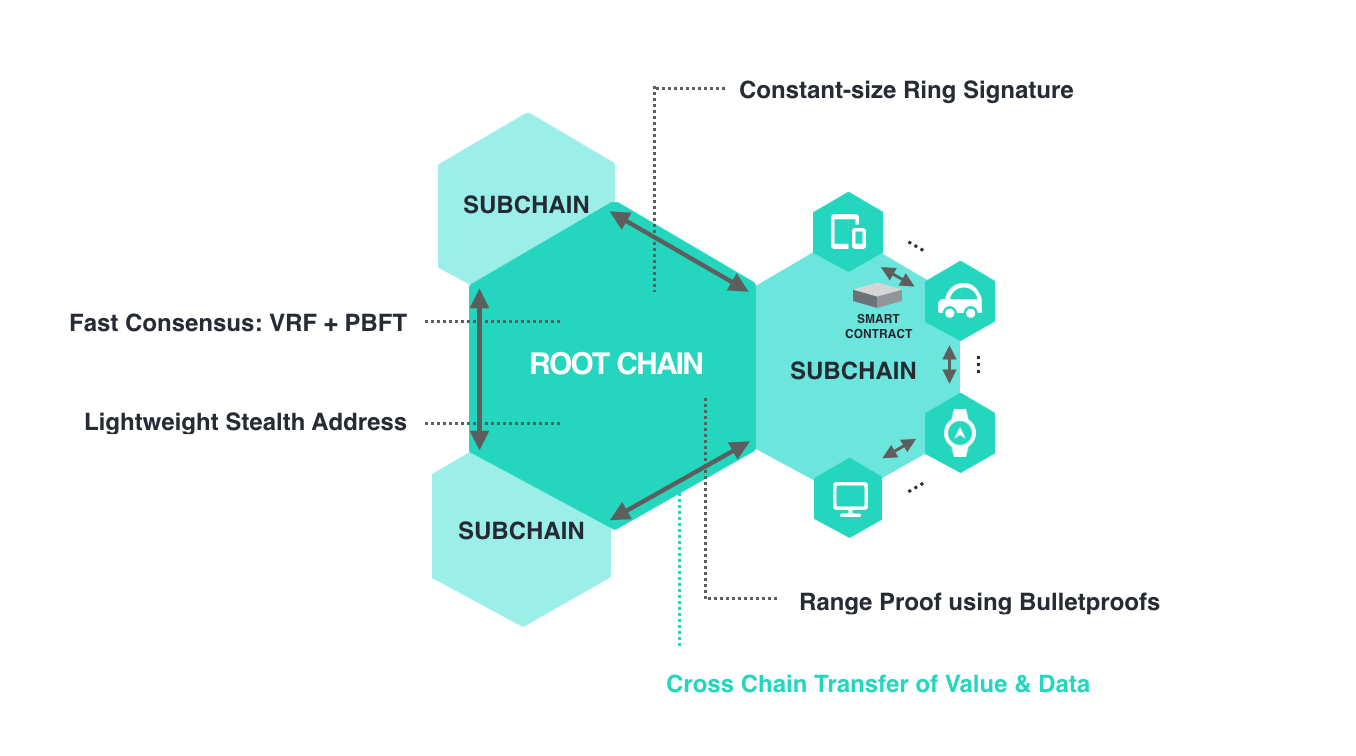
\includegraphics[width=\textwidth]{Figura1.png}
	\caption{IoTeX: Blockchain in blockchain, una architettura di rootchain con subchain}
\end{figure}

La blockchain radice è una blockchain pubblica accessibile da chiunque, che ha tre obiettivi principali:

\begin{enumerate}
	\item
	      \textbf{Inoltro} di valore e dati tra le subchain in modo da preservare la privacy per abilitare l'interoperabilità tra le subchain;
	\item
	      \textbf{Supervisione} delle subchain, ad esempio penalizzare gli operatori di subchain confiscando il deposito;
	\item
	      \textbf{Regolamento e ancoraggio} dei pagamenti e della fiducia per le subchain.
\end{enumerate}
Con questi obiettivi definiti, la rootchain si concentra in particolare su scalabilità, robustezza,
funzioni per preservare la privacy e capacità di controllare le subchain.
Una subchain, d'altra parte, potrebbe potenzialmente essere una blockchain privata e dipendere dalla rootchain per l'interazione con altre sottocatene. Una subchain richiede flessibilità
ed estendibilità per adattarsi ai diversi requisiti delle diverse applicazioni IoT. Una subchain sarà molto probabilmente gestita da operatori il cui ruolo è subordinato a un deposito di garanzia sufficiente, depositato sulla rootchain. Opzionalmente, il sistema consente agli operatori di nominare uno o più operatori che agiscono per suo conto, con o senza vincoli extra. L'operatore agisce come un client leggero nella rootchain, e come un nodo completo nella subchain per
confermare nuovi blocchi.
Nel complesso, le proprietà di rootchain e subchain sono riassunte in Tabella \ref{table:rootchainandsubchains}

\begin{table}[tp]%
	\caption{Confronto tra Rootchain e Subchain}
	\label{table:rootchainandsubchains}\centering %
	\begin{tabular}{l|l|l}
		\hline
		\textbf{Proprietà}          & \textbf{Rootchain}   & \textbf{Subchain}  \\
		\hline
		Pubblica vs Privata         & Pubblica             & Pubblica o Privata \\
		Scalabile                   & Necessario           & Varia              \\
		Robusta                     & Fortemente Richiesto & Richiesto          \\
		Incentrata sulla Privacy    & Richiesto            & Varia              \\
		Estendibilità               & Non-Turing completa  & Turing completa    \\
		Finalità Istantanea Blocchi & Richiesta            & Richiesta          \\
		\hline
	\end{tabular}
\end{table}

\subsection{Blockchain Root}
La blockchain root utilizza il modello basato su UXTO come Bitcoin \cite{21} e Monero \cite{20} per i seguenti motivi:

\begin{itemize}
	\item
	      L'ordinamento delle transazioni diventa banale, senza richiedere \emph{nonce} o
	      numeri di sequenza, il che pone richieste minime sugli schemi di consenso e permette di elaborare le transazioni in parallelo;
	\item
	      Applicando tecniche esistenti di conservazione della privacy come \emph{ring signature} e ZKSNARKs, diventa possibile nascondere il mittente, il destinatario e l'importo della transazione;
\end{itemize}

La blockchain radice è composta da blocchi collegati da hash, ed un blocco è costituito da  un'intestazione lo collega mediante un hash al blocco precedente, e da un elenco di transazioni.
La rootchain consente principalmente due tipi di transazione: (1) transazioni di base incluse
\texttt{P2PKH, P2SH, Multisig} e così via, e transazioni avanzate che consentono
operazioni tra blockchain come \texttt{BondedRegistration, Lock, ReLock, Reorg} ecc.. Le
transazioni validate vengono aggiunte ad un blocco che ha dimensione dinamica, con limite superiore di 8MB. Il nostro sistema di consenso produce un blocco ogni tre secondi come dettagliato
nella prossima sezione. La rootchain è progettata per essere non-Turning-Completa con il
supporto di uno script basato su stack e un ricco set di operazioni.

\pagebreak

\bibliography{bibliography}

\bibliographystyle{plain}

\end{document}